\documentclass[11pt,a4paper]{article}
\usepackage[utf8]{inputenc}
\usepackage[dutch]{babel}
\usepackage{pgfplots}
\usepgfplotslibrary{units}
\usepackage{float}
\usepackage{amsmath,amsthm}
\usepackage{amsfonts}
\usepackage{amssymb,marvosym}
\usepackage[left=2cm,right=2cm,top=2.5cm,bottom=2cm]{geometry}
\usepackage{graphicx}
\usepackage{multicol}
\usepackage{enumerate}
\usepackage{fancyhdr}
\pagestyle{fancy}
\usepackage{algorithm}
\usepackage{algpseudocode}
\usepackage{pgfplots}
\usepackage{multirow}
\usepackage{tikz}
\usetikzlibrary{arrows}
\usetikzlibrary{calc}

\floatname{algorithm}{Algoritme}


\usepackage[font=small,labelfont=bf]{caption}
\captionsetup[table]{aboveskip=-0.8em}
\captionsetup[table]{belowskip=-0.7pt}


\lhead {Proj. DAII: Genetische algoritmen} 
\chead{BAZ(~ \thepage ~ )NGA} 
\rhead{Robbert Gurdeep Singh}


\cfoot{} % get rid of the page number 

\usepackage{hyperref}
\usepackage{chngcntr}
\counterwithin*{section}{part}
\counterwithin{algorithm}{section}
\counterwithin{table}{section}
\counterwithin{figure}{section}

\hypersetup{
    colorlinks=false,
    pdfborder={0 0 0},
}

\author{Robbert Gurdeep Singh}
\title{{Project Algoritmen en datastructuren III}\\ \Huge Gedistribueerde Genetische algoritmen}
%\date{}



\pgfplotsset{compat=1.8}


\newcommand{\drawGraph}[4]{
\begin{tikzpicture}
\begin{axis}[scale only axis, 
	%x-as	
    xmin=0,
	xlabel=#1,	
	%y-as
	ylabel=#2,
	ymin=0,
	%Style
	height=5em,width=.37\textwidth,
	enlargelimits=0.05,
	grid=major,	legend pos=south east
]
#3
\end{axis}
\end{tikzpicture}
}


\newcommand{\lxaxis}[3]{\begin{tikzpicture}
\begin{axis}[scale only axis, 
cycle list name=exotic,
    xmode=log,
    log ticks with fixed point,
	%x-as	
	xlabel=#2,	
	%y-as
	ylabel=#1,
	ymin=0,
	%Style
	height=5em,width=.37\textwidth,
	enlargelimits=0.05,
	grid=major,	legend pos=south east
]
#3

\end{axis}
\end{tikzpicture}}

\newcommand{\rlxaxis}[3]{\begin{tikzpicture}
\begin{axis}[scale only axis, 
cycle list name=exotic,
    xmode=log,
    log ticks with fixed point,
	%x-as	
	xlabel=#2,	
	%y-as
	ylabel=#1,
	%Style
	height=5em,width=.37\textwidth,
	enlargelimits=0.05,
	grid=major,	legend pos=south east
]
#3

\end{axis}
\end{tikzpicture}}

\newcommand{\nxaxis}[3]{\begin{tikzpicture}
\begin{axis}[scale only axis,
cycle list name=exotic, 
	%x-as	
    xmin=0,
	xlabel=#2,	
	%y-as
	ylabel=#1,
	ymin=0,
	%Style
	height=5em,width=.37\textwidth,
	enlargelimits=0.05,
	grid=major,	legend pos=south east
]
#3

\end{axis}
\end{tikzpicture}}


\newcommand{\nxaxisr}[3]{\begin{tikzpicture}
\begin{axis}[scale only axis,
cycle list name=exotic, 
	%x-as	
	xlabel=#2,	
	%y-as
	ylabel=#1,
	ymin=0,
	%Style
	height=5em,width=.37\textwidth,
	enlargelimits=0.05,
	grid=major,	legend pos=south east
]
#3

\end{axis}
\end{tikzpicture}}

\newcommand{\rnxaxis}[3]{\begin{tikzpicture}
\begin{axis}[scale only axis, 
cycle list name=exotic,
	%x-as	
    xmin=0,
	xlabel=#2,	
	%y-as
	ylabel=#1,
	%Style
	height=5em,width=.37\textwidth,
	enlargelimits=0.05,
	grid=major,	legend pos=south east
]
#3

\end{axis}
\end{tikzpicture}}


\newcommand{\rnxaxisr}[3]{\begin{tikzpicture}
\begin{axis}[scale only axis, 
cycle list name=exotic,
	%x-as	
	xlabel=#2,	
	%y-as
	ylabel=#1,
	%Style
	height=5em,width=.37\textwidth,
	enlargelimits=0.05,
	grid=major,	legend pos=south east
]
#3

\end{axis}
\end{tikzpicture}}


\newcommand{\itemMB}[1]{
	\item[$\boldsymbol{#1}$:]
}

\newcommand{\itembf}[1]{
	\item \textbf{#1}:
}



\newcommand{\abs}[1]{
	\lvert #1 \rvert
}

\newcommand{\addploti}[1]{\addplot table [y=i, x=testValue, col sep=comma] {../../tests/param_results/#1.log};}
\newcommand{\addplotf}[1]{\addplot table [y=f, x=testValue, col sep=comma] {../../tests/param_results/#1.log};}
\newcommand{\addplott}[1]{\addplot table [y=t, x=testValue, col sep=comma] {../../tests/param_results/#1.log};}

\definecolor{mymark}{HTML}{EBB8B8}

\begin{document}

\twocolumn[\begin{@twocolumnfalse}
    \maketitle
    
    \begin{abstract}
    	{\em
    	In dit verslag bespreken we de implementatie van een genetisch algoritmen. We onderzoeken wat de optimale parameters zijn en vergelijken enkele algoritmen.
    	}
    \end{abstract}
    
\end{@twocolumnfalse}]

Om ons algoritme te parallelliseren gaan we parallel meerdere keren naast elkaar het algoritme uitvoeren zoals beschreven in sectie \ref{ssub:genetic}. Als we echt gebruik willen maken van parallelle rekenkracht, dan moeten we die processen natuurlijk met elkaar laten communiceren.   In de volgende secties bespreken we wat en hoe we zullen communiceren.
\section{Idee}
\label{sec:idee}
In de grafieken van figuur \ref{graf:numLovers} zien we dat hoe meer individuen we hebben, hoe minder iteraties er nodig zijn maar ook hoe groter de uitvoeringstijd. Nu kunnen we een grotere populatie bestaande uit verschillende deelpopulaties nabootsen. Elke deelpopulatie geven we zijn eigen processor.  

%todo
We merken op dat individuen gekozen door een positieve Touranament Selection\footnote{zie sectie \ref{sec:positiveTournament} en \ref{sub:tournament}} ideaal zijn om gedeeld te worden over processen heen. We zullen op zo'n manier individuen selecteren uit de populatie van het huidige proces en die injecteren in de populaties van de andere processen. 

\section{Algoritme}


\begin{figure}[H]
\centering
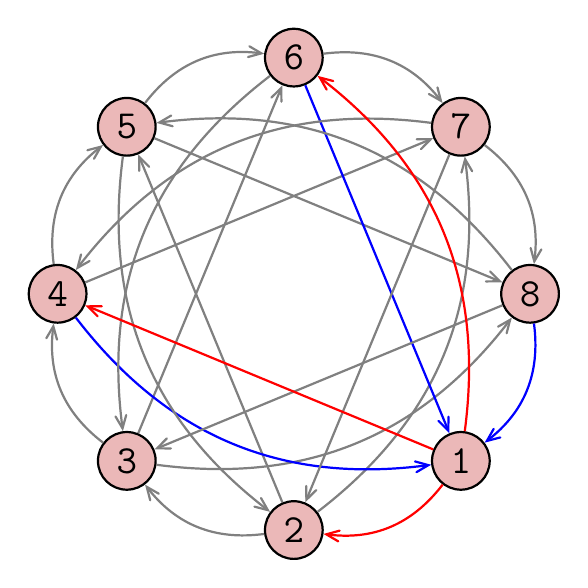
\begin{tikzpicture}[->,>=angle 45,shorten >=0pt,auto,node distance=2cm,
  thick,main node/.style={circle,fill=mymark,draw,font=\ttfamily\Large}]


  
  \foreach \a in {1,2,...,8}{
  \node[main node] (\a) at (\a*-360/8: 3cm) {\a};
}


  \path[every node/.style={font=\sffamily\small}]
(2)	edge [draw=black!50,bend left] node [] {} (3)
	edge [draw=black!50] node [] {} (5)
	edge [draw=black!50,bend right] node [] {} (7)
(3)	edge [draw=black!50,bend left] node [] {} (4)
	edge [draw=black!50] node [] {} (6)
	edge [draw=black!50,bend right] node [] {} (8)
(4)	edge [draw=black!50,bend left] node [] {} (5)
	edge [draw=black!50] node [] {} (7)
	edge [draw=blue,bend right] node [] {} (1)
(5)	edge [draw=black!50,bend left] node [] {} (6)
	edge [draw=black!50] node [] {} (8)
	edge [draw=black!50,bend right] node [] {} (2)
(6)	edge [draw=black!50,bend left] node [] {} (7)
	edge [draw=blue] node [] {} (1)
	edge [draw=black!50,bend right] node [] {} (3)
(7)	edge [draw=black!50,bend left] node [] {} (8)
	edge [draw=black!50] node [] {} (2)
	edge [draw=black!50,bend right] node [] {} (4)
(8)	edge [draw=blue,bend left] node [] {} (1)
	edge [draw=black!50] node [] {} (3)
	edge [draw=black!50,bend right] node [] {} (5)
(1)	edge [draw=red,bend left] node [] {} (2)
	edge [draw=red] node [] {} (4)
	edge [draw=red,bend right] node [] {} (6)

;
\end{tikzpicture}
\caption{Punten binnen en buiten de figuur \texttt{soos.poly} met snijpunten.}
\end{figure}


\begin{figure}[H]
\centering
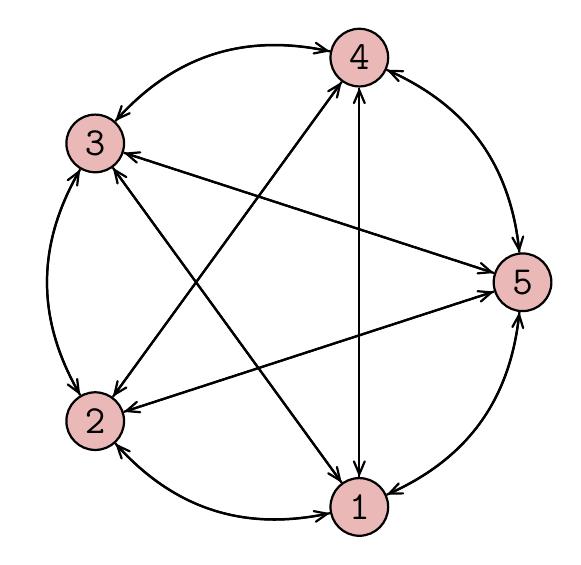
\begin{tikzpicture}[->,>=angle 45,shorten >=0pt,auto,node distance=2cm,
  thick,main node/.style={circle,fill=mymark,draw,font=\ttfamily\Large}]

\foreach \a in {1,2,...,5}{
  \node[main node] (\a) at (\a*-360/5: 3cm) {\a};
}



  \path[every node/.style={font=\sffamily\small}]

(1)	edge [bend left] node [] {} (2)
	edge node [] {} (3)
	edge node [] {} (4)
	edge [bend right] node [] {} (5)
(2)	edge [bend left] node [] {} (3)
	edge node [] {} (4)
	edge node [] {} (5)
	edge [bend right] node [] {} (1)
(3)	edge [bend left] node [] {} (4)
	edge node [] {} (5)
	edge node [] {} (1)
	edge [bend right] node [] {} (2)
(4)	edge [bend left] node [] {} (5)
	edge node [] {} (1)
	edge node [] {} (2)
	edge [bend right] node [] {} (3)
(5)	edge [bend left] node [] {} (1)
	edge node [] {} (2)
	edge node [] {} (3)
	edge [bend right] node [] {} (4)




;
\end{tikzpicture}
\caption{Punten binnen en buiten de figuur \texttt{soos.poly} met snijpunten.}
\end{figure}

 % \node[main node] (1) {1};
 % \node[main node] (2) [below right of=1] {2};
 % \node[main node] (3) [below of=2] {3};
 % \node[main node] (5) [below left of=1] {4};
 % \node[main node] (4) [below of=5] {5};
% section  (end)
\section{Bronnen}
Er moet vermeld worden dat het icosagon bestand afkomstig is van Jonathan Peck. 

\end{document}